
% =========================================================================
\begin{quotation}
  ``To understand brain function, the focus of [our] investigations must expand
  from detailed responses and structure of single cells to include unit
  responses to the activity of other cells, and how these responses are
  distributed over a population of similar cells as wells as across populations
  of different cells.''  - \textit{\citet[p.]{Shamma:1998}}
\end{quotation}
\yellownote{Get page number of this quote}
% =========================================================================

%===================================
\section{Introduction    \label{sec:CN:introduction}}

Shihab Shamma calls upon the science community, particularly members of its
physiology and neuroscience subgroups, to investigate the role of populations of
neurons and to pay attention to the role of populations of neurons in
neurophysiology.  This chapter draws on the wealth of experimental data
accumulated in auditory neuroscience to create a detailed, \BNN model of the
cochlear nucleus stellate cell network.  The design and methods for the
construction of the model shall provide insights relevant to other neural
network models of the brain, especially those that use highly-specific sensory
pathways.

% \smallskip{}
It still remains a laborious task to develop an accurate representation of
complex behaviour of real neural networks.  Pre-eminent computational
neuroscientists have noted that ``choices, assumptions, and guesses [are] an
integral part of neuronal modeling'' \citep{SegevBurkeEtAl:1998}.  With the
acceleration of computational power and enhanced experimental techniques in
multi-unit recordings are enabling more detailed neural models to be developed.
There is much to be gained from biophysically-realistic modelling approaches,
especially in the heavily investigated cochlear nucleus of mammals and highly
evolved auditory systems of bats and birds.


%\yellownote{See  neural detail in auditory system\citep{LuRubioEtAl:2008}}

% \smallskip{}

% {Discuss use of Poisson models vs HH-like models.  Discuss single cell
% simulation vs whole network simulation during optimisation.}
To develop and optimise detailed neural models and neural network models,
reproducible research methods are required.  Examples of parameter estimation
and fitting in neural models are also becoming more advanced, for example
SSNNS~\citep{SichtigSchafferEtAl:2008}, NeuroFitter
\citep{VanAchardEtAl:2007}~and MultiRunFitter (a feature in NEURON).  In this
chapter, a tabular method introduced by \citet{NordlieGewaltigEtAl:2009} is used
to summarise the neural models used in each optimisation step.  The Nordlie
tables shown in each optimisation stage consist of A) the model summary, B) cell
type populations, C) connectivity between two cell types, D) neuron and synapse
models, and E) optimisation parameters.  This method aims to show a consistent
and recognisable format for presenting various neural network models and their
constituents.
%\yellownote{this needs more explanation in the methods sections}

% \smallskip{}

The standard methods for optimisation can be simply described with the following
steps: \begin{enumerate}
\item specify function or model we want to optimise
\item specify criterion we want to satisfy
\item specify the parameters that will be adjusted, and any constraints on those
  parameters and finally
\item perform the optimization.
\end{enumerate}

In attempting to create a realistic microcircuit the parameter optimisation
routine, these steps need to be reiterated in sequential stages.  The parameters
chosen in the sequential optimisation stages should be chosen so that they do
not influence the properties of previously fitted parameters.

% \smallskip{}

In this chapter, the connections within the mammalian cochlear nucleus stellate
network (Figure~\ref{fig:microcircuit}) are developed using a sequential method
of optimisation steps.  The parameters of each cell type are determined based on
experimental data or are optimised based solely on responses to simple stimuli.


Each cell type is shown with its \EIRA and \PSTH, although this may vary within cell types.
\yellownote{Explain the figure more thoroughly}

The stellate network model drawn in Figure~\ref{fig:microcircuit} describes the
following cells and models:
\begin{enumerate}
\item The auditory model: The Carney phenomenological auditory model
  \citep{ZilanyBruceEtAl:2009} provides spiking input to cochlear nucleus
  neurons across frequencies and spontaneous rate types of the auditory nerve
  from an arbitrary input stimulus.  The base line in
  Figure~\ref{fig:microcircuit} is a simplification of auditory nerve fibres
  (ANF) from low best frequency (BF) to high BF (left to right).  The model
  reproduces responses for high and low SR ANFs at 100 channels across the
  frequency range 200 Hz to 48 kHz.
\item The Golgi cell: a {GABA}ergic \VCN~marginal shell unit that is presumed to
  regulate excitability in the \GCD~and core \VCN~units
  \citep{FerragamoGoldingEtAl:1998}.  Only one \textit{in vivo} study has
  recorded extracellular data in the marginal shell area of the
  \CN~\citep{GhoshalKim:1997}.  The presumed characteristics of Golgi cells are
  taken from that study and are defined by a monotonic response to tones and
  noise, a type I\slash III~\EIRA, and an unusual or chopper {\PSTH}.
\item The D~stellate cell: a glycinergic, large multipolar cell with
  \OnC~\PSTH~response that acts as a coincidence detector.  Its large dendritic
  area increases its response to noise allowing it to behave as a wide-band
  inhibitor in the \VCN, \DCN, and
  contralateral\CN~\citep{SmithMassieEtAl:2005,ArnottWallaceEtAl:2004,NeedhamPaolini:2007}.
\item The Tuberculoventral cell: a glycinergic, type II~{\EIRA}~unit in the deep
  layer of the \DCN~\citep{SpirouDavisEtAl:1999}.  This cell acts as a delayed
  echo-suppressor and narrow-band inhibitor, with recurrent connections between
  D~and T~stellate cells in the
  \VCN~\citep{Alibardi:2006,OertelWickesberg:1993,WickesbergWhitlonEtAl:1991}.
\item The T~stellate cell: one of the major output projection cells of the
  cochlear nucleus to the inferior colliculus.  This multipolar neuron has been
  shown to have robust spectral representation and enhanced synchronisation to
  modulation in speech
  sounds~\citep{BlackburnSachs:1990,KeilsonRichardsEtAl:1997}.
\end{enumerate}

\begin{figure}[htb]
  \centering
  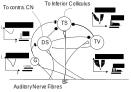
\includegraphics[width=\textwidth]{CNcircuit}
  \caption[Cochlear nucleus stellate microcircuit]{Cochlear nucleus stellate
    microcircuit (see text for details). }
  \label{fig:microcircuit}
\end{figure}


% \smallskip{}

Optimisation of a detailed \BNN~model requires a realistic input model with
which to mimick the behaviour experimentally observed in live neural
networks. The input to the CN stellate model, the auditory nerve fibres, is
discussed in the next section. To further fit the parameters of the CN model, a
simplistic and sequential method is applied to each of the cell-types using
experimental data.

\yellownote{This para is about pushing the reader towards
  the following sections.  I'm not sure about the assertion of 'well-tested':
  too narrative, less science-y.  Needs to expand on reasons for wanting to
  create a biophysically realistic model of the CN. Discuss reason for using
  whole network in TV and TS optimisation. }


%===================================
\section{Auditory System    \label{sec:CN:auditory-model}}

Advanced auditory fidelity and localisation is an exceptional feature of hearing
perception in animals.  This speciality works to a high degree despite the input
at the round window of the cochlea being one dimensional and very noisy.
Modelling in the auditory periphery has benefited extensively from the work of
Liberman, Greenwood, Patterson, Young, Sachs and others, in acoustic \textit{in
  vivo} experiments.  Models of the auditory system over the last 30 years have
expanded our understanding of the mechanical processes in the middle ear and
cochlea, and the specialised synapse between the inner hair cell and the
auditory nerve~\citep{DavisVoigt:1991,Carney:1993,MeddisHewittEtAl:1990}.

% \smallskip{}

The auditory system is topographically ordered from the basilar membrane to the
cortex in terms of frequency selectivity, also called
tonotopicity~\citep{YoungOertel:2004}.  The population of auditory nerve fibres
(ANFs, Fig.~\ref{fig:CN_Cat_Human}) bifurcate after entering the cochlear
nucleus to innervate the \VCN~and \DCN, retaining their tonotopic order
\citep{Lorente:1981,Liberman:1982,Liberman:1993}.  Type 1 \ANFs are categorised
into {\HSR}~and {\LSR}~fibres \citep{Liberman:1978}, where \LSR~fibres have a
higher threshold and wider dynamic range than \HSR~fibres.  They also project to
the \GCD~\citep{RyugoParks:2003, RyugoHaenggeliEtAl:2003} along with the
smaller, unmyelinated type 2 \ANFs, which suggests they play a different role in
sound processing to \HSR~fibres.

% \smallskip{}

\begin{figure}[htb]
  \begin{center}
    \resizebox{2.25in}{!}{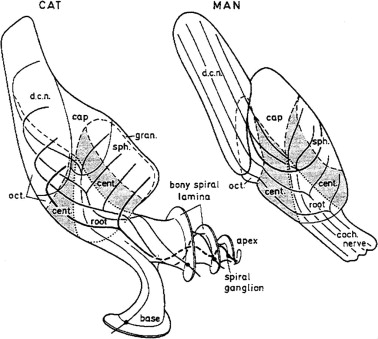
\includegraphics[width=2.25in,keepaspectratio]{Cat_Human_CN}}
    \caption[Tonotopic innervation by ANFs in the CN of man and cat.]{Cochlear nucleus innervation by ANFs follows the same tonotopic organisation in man and cat
\citep{RyugoParks:2003,Ryugo:1992,Spoendlin:1973}. (Image reprinted from \citep{})}
    \label{fig:CN_Cat_Human}
  \end{center}
\end{figure}


% \smallskip{}

\yellownote{Auditory model and history should be in the METHODS section.}
%A paragraph on the history of AN modelling \citep{LeakeSnyderEtAl:1993, ArnesenOsen:1978, CloptonWinfieldEtAl:1974}.  Perhaps Rose et al 1959 would be better suited here}

%
% \smallskip{}

In examining the properties of a detailed neural model of the cochlear nucleus, a realistic and phenomenologically sound auditory model is needed to represent sounds and transformations that occur in the central auditory system.

%
% \smallskip{}






%===================================
\subsection{Auditory nerve fibre model   \label{sec:CN:resp-audit-models}}

The auditory nerve inputs to the cochlear nucleus model neurons are provided by
phenomenological auditory periphery models originating from \citet{Carney:1993},
the ARLO model \citep{HeinzZhangEtAl:2001}, the Bruce model
\citep{BruceSachsEtAl:2003, ZilanyBruce:2006, ZilanyBruce:2007}, and the Zilany
model \citep{ZilanyBruceEtAl:2009}.  The AN model consists of an outer\slash
middle ear pre-processing filter, a cochlea filterbank, IHC-to-AN synapse model
and dead-time modified Poisson spike generator, as shown in
Fig.~\ref{fig:ZilanyBruceFig}.  \citet{HeinzZhangEtAl:2001} incorporated cochlea
filters based on the critical bandwidths obtained from psychophysical
experiments in humans.  The ARLO model of the cat auditory periphery, with
non-linear compression and two-tone suppression, is used in this study except in
the vowel simulation where the human auditory periphery model is used.
\yellownote{TODO: AN model paragraph has been changed - fix any comment related
  to new Zilany}

% \smallskip{}

% The \citet{ZilanyBruce:2007} model improves the previous AN model by an
% additional signal path and its predictions have matched a wide range of
% physiological data in normal and impaired cat data. The most recent AN model
% comprises an power-law synapse model, with internal $1/f$ noise, that enhances
% the behaviour of long-term dependence in ANFs \citep{ZilanyBruceEtAl:2009}.

% \smallskip{}

\yellownote{Why is it the cat model? updating Carney model? Updating of the
  Carney auditory model has led to the change in the model's configuration from
  an original implementation of the rat model.  The default species is the cat
  and will be used in the data presented in this chapter.}

\begin{figure}[htb]
  \begin{center}
    \resizebox{3.5in}{!}{\includegraphics[keepaspectratio=true]{NoFigure}}
    % \resizebox{\textwidth}{!}{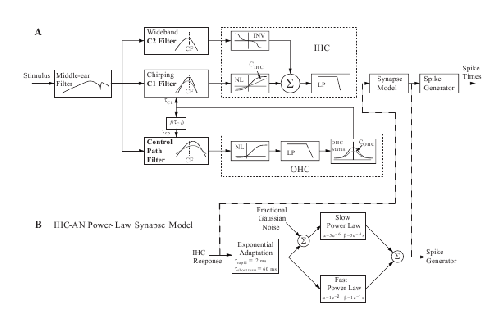
\includegraphics[keepaspectratio=true]{gfx/ZilanyCarney-JASA-2009-Fig2.eps}}
    \caption[Auditory periphery model]{Auditory periphery model with dual power-law synapse \citep[originally printed in ][]{ZilanyBruceEtAl:2009}.
\yellownote{if this figure is used it needs permission by the original authors}
\label{fig:ZilanyBruceFig}}
  \end{center}
\end{figure}


\todo[inline]{Explain Figure \ref{fig:Compression}}

\begin{figure}[htb]
  \centering
  \subfloat[][Cat audiogram]{\resizebox{3.5in}{!}{\includegraphics[keepaspectratio=true]{CatAudiogram}}}
  \subfloat[][Rat audiogram]{\resizebox{3.5in}{!}{\includegraphics[keepaspectratio=true]{RatAudiogram}}}
  \caption{Compression in the Bruce and Zilany AN model for cat (A) and rat (B).}
  \label{fig:Compression}
\end{figure}



%===================================
\subsection{Spiking in Poisson neural models}

The neural models used in the auditory nerve fibres and Golgi cell model are
inhomogeneous Poisson processes.  The instantaneous rate is passed through the
Jackson spiking model, which includes refractory effects typical of the auditory
nerve fibres \citep{Jackson:2003,JacksonCarney:2005}.  Spike trains for each
neuron in the model are created at the start of each repetition of the stimulus,
but can be saved and loaded from file.



% \yellownote{TODO: serious reworking to be done here}

% Analysis of the frequency
% response area of ANF generates known parameters for each fibre, these are:
% \begin{itemize}
% \item the spontaneous rate (SR), generated in silence and is
%   categoried into two groups High SR ($>$18 sp/s) and Low SR ($<$ 18
%   sp/s);
% \item threshold, the sound pressure level(SPL) at which the cell
%   responds above the spontaneous rate
% \item characteristic frequency (CF)
% \end{itemize}

% \smallskip{}



% \begin{figure}[tbh]
%   \begin{center}
% % \resizebox{3.5in}{!}{\includegraphics[keepaspectratio=true]{NoFigure}}
% % \resizebox{3.5in}{!}{\includegraphics[keepaspectratio=true]{ClickDelay}}
%     \caption{Response of AN and CN cells to click stimuli. }
%     \label{fig:ClickDelayAN}
%   \end{center}
% \end{figure}

%===================================
\section{Cochlear Nucleus Stellate microcircuit \label{sec:CN:cochl-nucl-stell}}

\subsection{CN neural models}

Single-compartment Hodgkin-Huxley-like neural models were used for the neural
models.  The current models in each of the cell types of the cochlear nucleus
stellate network were originally presented by \citet{RothmanManis:2003b}.


Type I-c classic regular firing type contains a voltage-activated sodium, high
threshold potassium, and hyperpolarisation mixed-cation, and leak current
channels.  This neural model an integrator and is strongly influenced by the \Ih
current, which is active at rest.  Type I-t transient regular firing type is
similar to the Type 1 classic but with A-type potassium current channels.
A-type potassium channels are unique to the cochlear nucleus, particularly to T
stellate cells \citep{RothmanManis:2003,RothmanManis:2003a}.  D-stellate cells
contain low-threshold potassium current channels, which is strongest in bushy
cells, to enhance response to coincident inputs.


\yellownote{Discuss RM model (put in Methods Chapter).  Perhaps expand more on
  the role of the currents on each neuron in the CN model.}  



%===================================
\subsection{Synapse Models}

\yellownote{TODO. THis is inlcuded in the GA chapter, but it should go in the  Methods chapter}



%===================================
\subsection{Topological definitions and limitations    \label{sec:CN:tonot-conn}}

Tonotopic connectivity in the stellate cochlear nucleus model is defined by the
regular organisation of afferent ANFs into distinct iso-frequency channels.  The
channels are separated using even spatial distance (based on the basilar
membrane and auditory nerve separation) with centre frequency calculated by the
Greenwood function for the cat
\citep[see~\ref{tab:ModelSummary},][]{Greenwood:1990}.  The HSR terminals of
individual fibres generally cover 70 $\mu$m and LSR fibres 100 $\mu$m in mice
\citep{OertelWuEtAl:1988,OertelWu:1989}.

%\yellownote{and the dendrites of finely-tuned neurons (bush and T stellate cells) generally}

Figure~\ref{fig:CNconn} shows the method for Gaussian spread of connections
between cell types in the \CN\@.  The \CF of the CN channels are separated using
the same Greenwood function as used for the AN filterbank.


% \smallskip{}


% \begin{figure}[htb]
%   \begin{center}
% %\resizebox{3.5in}{!}{\includegraphics[keepaspectratio=true]{NoFigure}}
% \resizebox{0.85\textwidth}{!}{\includegraphics[keepaspectratio=true]{CNConn}}
%     % \resizebox{0.8\textwidth}{!}{\input{./gfx/CNConn.tex}}
%     \caption{Cochlear nucleus network model diagram \label{fig:CNdiagram%   \end{center}
% \end{figure}



\begin{figure}[htb]
  \begin{center}
    % \resizebox{3.5in}{!}{\includegraphics[keepaspectratio=true]{NoFigure}}
    \resizebox{\textwidth}{!}{\includegraphics[keepaspectratio=true]{gfx/CNConn}}
    % \resizebox{0.8\textwidth}{!}{\input{./gfx/CNConn.tex}}
    \caption{Gaussian connection between cell types in cochlear nucleus stellate network.}
    \label{fig:CNconn}
  \end{center}
\end{figure}

% \smallskip{}

Extrinsic parameters that control the connectivity between two cell-type groups
can be defined by:
\begin{itemize}
\item $d_{\textrm{{Pre}}\to\textrm{{Post}}}\xspace$ is the temporal delay
  between a pre-cells' AP trigger and the onset of the post-synaptic current.
  This delay incorporates the axonal conduction delay and diffusion time across
  the synaptic cleft.
\item $w_{\textrm{{Pre}}\to\textrm{{Post}}}\xspace$ is the synaptic weight of
  the post-synaptic current influx caused by the pre-cells' neurotransmitter
  activating the receptor channels of the post-synaptic cell.  This value is the
  same for all synapses in this connection type.
\item $n_{\textrm{{Pre}}\to\textrm{{Post}}}\xspace$ is the number of presynaptic
  cell type synapses onto individual cells in the post-synaptic cell type.
\item $s_{\textrm{{Pre}}\to\textrm{{Post}}}\xspace$ is the spatial or feature
  specific spread of connections from presynaptic cells onto post-synaptic
  cells.  The spread is the variance of a Gaussian probability distribution,
  $\mathcal{N}(i,\sqrt{s})$, representing the probability of the post-synaptic
  cell in position $i$ receiving input from a post-synaptic cell in the
  network's discrete slices; in this case frequency channels.  The spread
  variable is uniform across the stellate CN network.  A spread of 0 means all
  connections come from the same frequency channel, assuming no offset.
\item $o_{\textrm{{Pre}}\to\textrm{{Post}}}\xspace$ is the offset in
  distribution of connections between presynaptic cell types and post-synaptic
  cell.  The offset variable adjusts the centre point of the probability
  distribution, $\mathcal{N}(i + o, \sqrt{s})$, away from the post-synaptic
  cell's position $i$.
\end{itemize}

%\yellownote{New limitations of place-based connectivity}

The creation of neural microcircuits based on ``place'' is easily amenable to
different sensory neural network models; however there are problems and unique
features that may be necessary to ensure realistic representation of the system.
The unique unit of the network is the place-channel or feature-channel of the
microcircuit.  In this model it is the iso-frequency-channel that receives
afferent input from the narrowest receptive field possible in the auditory nerve
model.

Connection variables between cell-types are generally uniform across the network
but may be adjusted to suit the model.  Model parameters may be different
between species or within species, therefore, without adequate information
regarding exact neuron to neuron connection reasonable assumptions are made
based on the average population data.  Issues arise at the ends of large-scale
topographic BNNs with overlapping place\slash channel connections.  Boundaries
are considered closed bookends, where post-synaptic neurons select only from
those with its connection range.  The best modelling behaviour would arise,
therefore, in the middle sections.


% \section{Simulations}

% \yellownote{ }
% Optimisation simulations were designed to be performed on either a single PC or a parallel architecture system.


% %The random number generator used was the internal RNG of NEURON, MCellRand4 



% The simulation for each optimisation routine the integration timestep was 0.1 ms    parameters
\yellownote{A generic section called 'Simulations' was proposed to go here.
  This would state the integration timestep, the system used, the RNG used etc.
  This could perhaps go in the Methods chapter}


%%% Local Variables:
%%% mode: latex
%%% mode: tex-fold
%%% mode: visual-line
%%% TeX-master: "SimpleResponses"
%%% TeX-PDF-mode: nil
%%% End:
